\documentclass[../../../main]{subfiles}
\begin{document}
\subsection{Theory}
\label{sub:Theory}

This subsection is dedicated to explaining the theory to what a Qqadrature encoder is and what it does. \\
A Quadrature Encoder uses two channels to sense the position of, typically, a rotating disk/shaft or a linear strip. The disk or strip has two paths on it, positioned 90 degresse out of phase of eachother, see figure \ref{rotary_encoder}. Stationary sensors are placed, so that when the tracks moves the sensors produces a output signal depending on the part of the track that is visible. The output consits of two outputs, one for each track/channels, typically called A and B, see figure \ref{channels_1}

\begin{figure}[H]
  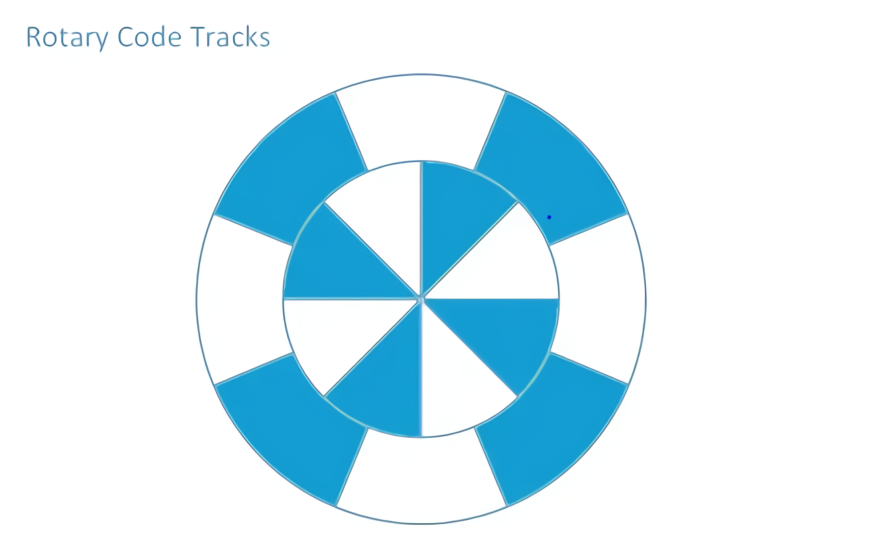
\includegraphics{pictures/encoder.png}
  \caption{The figure shows the tracks of a rotary encoder.}
  \label{rotary_encoder}
\end{figure}

\begin{figure}[H]
  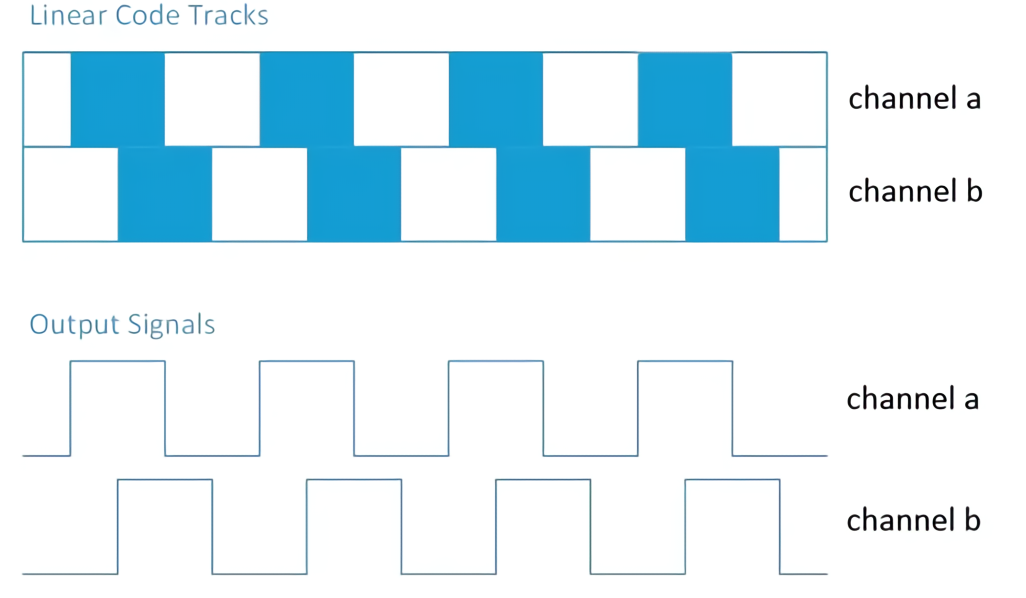
\includegraphics{pictures/channels.png}
  \caption{This figure shows the two channels and logic output of them}
  \label{channels_1}
\end{figure}

The Quadrature Decoder is the one interpreting the output signals created by the Quadrature Encoder. It determines how far the apparatus has moved, since last movement, by counting the transitions on the two channels. It uses the same princip to determine the direction of the movement. As it can be seen on figure \ref{channels_1}, the pattern for a clockwise movement is channel A going high before B and wise versa for counter clockwise.

\end{document}
